\subsection{K-Means}
We have tested on each dataset 57 different configurations of the K-Means algorithm, by using the 3 different distance metrics with 19 different values of the k (from 2 to 20). For each of these configurations, we have run the K-Means 10 times, in order to account for the randomness of the centroid initialization. This results in a total of 570 runs of the K-Means algorithm for each dataset. From the evaluation metrics extracted for each of these runs, we study the effect of each of the 2 hyperparameters and study the best performing runs according to each of the metrics.

\subsubsection{Hyperparameter Study}
Before starting with the study of the best runs themselves, let us first observe some preliminary patterns about the measured metrics and the effect of each hyperparameter on the clustering performance.

In Figure \ref{fig:metrics_corr} we summarize the relationship between the different metrics that were measured for two datasets. Each is a matrix plot where the lower triangle is a heatmap of the Pearson correlations between each pair of metrics, the diagonal elements are the histogram distributions of values of each metric, and the upper triangular has for each pair of metrics the plot of their values for all runs. It is interesting to observe that, while we would expect all of the metrics to agree on the identified trends, there are some cases where the opposite behavior is displayed.(the plots can be found in the \texttt{code} floder).

\begin{figure}[h!]
    \centering
    \begin{subfigure}{0.49\textwidth}
        \centering
        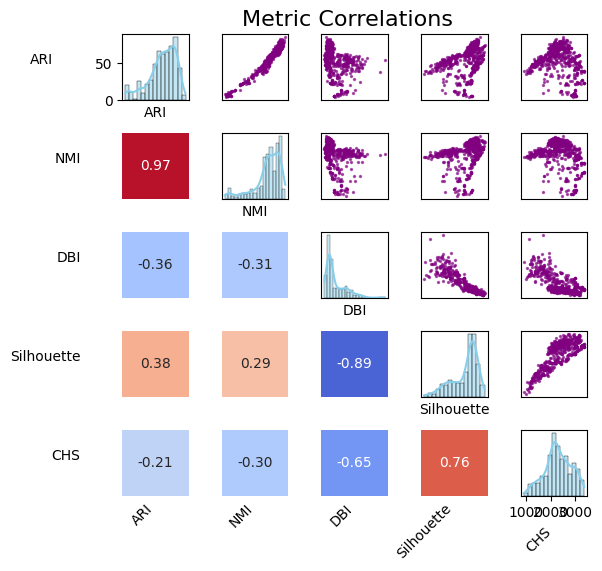
\includegraphics[width=\linewidth]{figures/KMeans/penbased_metrics_correlations_matrix.png}
        \caption{Pen-based metric correlations}
    \end{subfigure}
    \hfill
    \begin{subfigure}{0.49\textwidth}
        \centering
        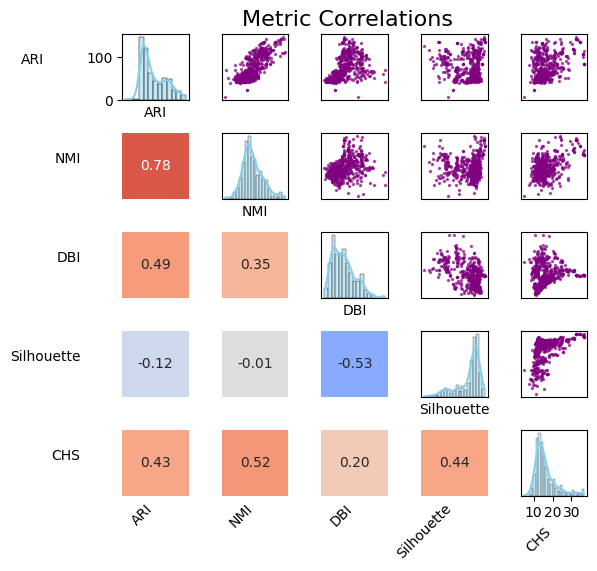
\includegraphics[width=\linewidth]{figures/KMeans/hepatitis_metrics_correlations_matrix.png}
        \caption{Hepatitis metric correlations}
    \end{subfigure}
    \caption{Metric correlations and distributions in two datasets}
    \label{fig:metrics_corr}
\end{figure}

Parallelly, a different set of interesting relationship are displayed in Figure \ref{fig:pairplot}, where we can see heatmaps of the ARI and the Time across the different pairwise hyperparameter configurations. We can observe a general trend regarding execution time: it seems to have considerably larger values for the Clark distance metric compared to those of the other 2, which reflects the higher computational cost that this distance metric has. Additionally, we see a noteworthy divergence in the ARI trends: in the Pen-based dataset (which has 10 classes), bigger values of k (greater than 7) seem to achieve the best scores, with a somewhat lower performance with the Clark distance than with the other two; meanwhile, in the Hepatitis dataset (which has 2 classes), lower values of k seem to achieve a better ARI, with a significantly better performance with the Clark distance metric than with the other two. The behavior with respect to the k was to be expected due to the true number of labels of each dataset, yet it still is compelling to see it reflected so clearly in the results. On the other hand, it is enlightening to see opposite behavior with respect to the distance metric, which reflects that the Clark distance fails to capture some properties of the Pen-based dataset, while it excells to do so within the Hepatitis dataset.

\begin{figure}[H]
    \centering
    \begin{subfigure}{0.49\textwidth}
        \centering
        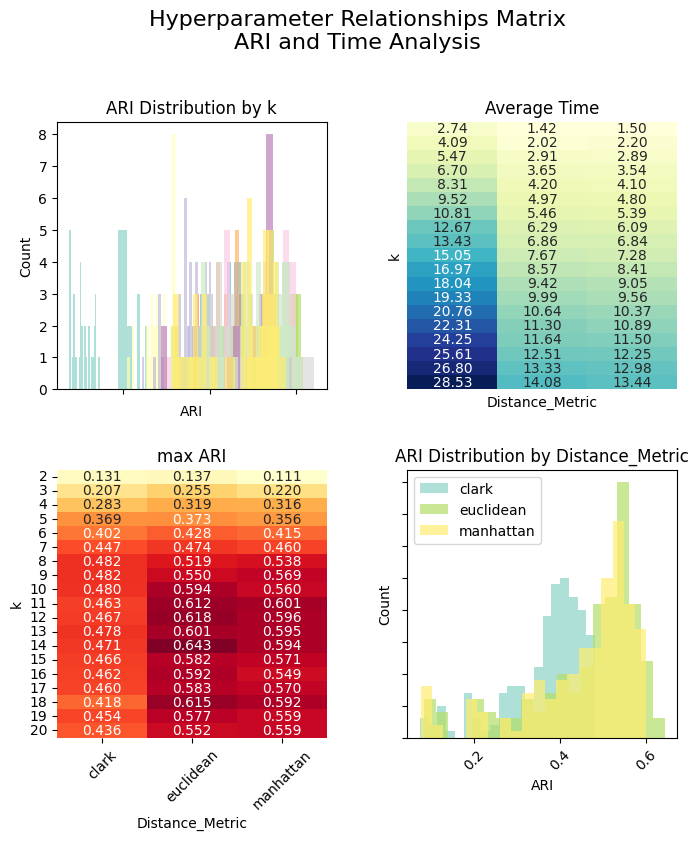
\includegraphics[width=\linewidth]{figures/KMeans/penbased_hyperparameter_pairplot_matrix.png}
        \caption{Pen-based pairplot matrix}
    \end{subfigure}
    \hfill
    \begin{subfigure}{0.49\textwidth}
        \centering
        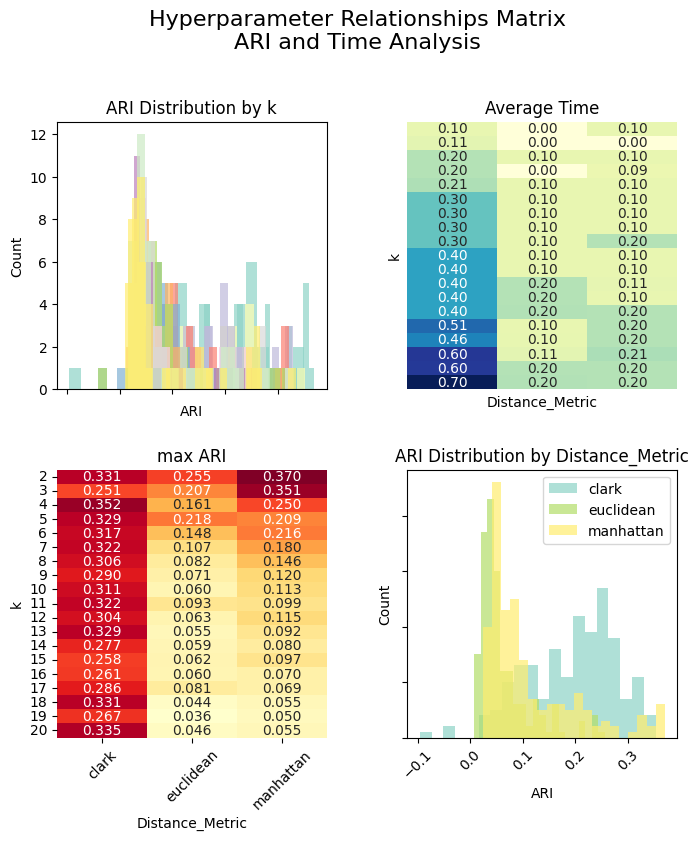
\includegraphics[width=\linewidth]{figures/KMeans/hepatitis_hyperparameter_pairplot_matrix.png}
        \caption{Hepatitis pairplot matrix}
    \end{subfigure}
    \caption{Hyperparameter pairplot matrices based on F1 Score and Time}
    \label{fig:pairplot}
\end{figure}

\subsubsection{Best Runs}

